\chapter{Geheugenbeheer}

Een van de belangrijkste taken die het besturingssysteem heeft, is het beheer
van het werkgeheugen. Het besturingssysteem moet kiezen waar de programma's in
het geheugen terecht komen, hoeveel geheugen elk programma toegewezen krijgt,
welke stukken code aan welke stukken geheugen mogen komen, enz. Er zijn
verschillende strategie\"en mogelijk om het geheugen te beheren, elk met zijn
voor- en nadelen.

\TODO{tekeningen toevoegen aan dit hoofdstuk}

\TODO{misschien definitie geven van logisch en fysiek adres?}

\section{Segmentatie}

In het vak Computersystemen werd er al een vorm van geheugenbeheer besproken:
\emph{segmentatie}. Een programma wordt hierbij in verschillende stukken
gebroken --- \emph{segmenten} --- die elk logisch bij elkaar horen. Zo kan er bijvoorbeeld een
codesegment zijn waar alle instructies van het programma in staan. Het
datasegment bevat dan weer de data van de applicatie, en het stapelsegment bevat
de data die het programma op de stapel opslaagt. De Intel x86-processor biedt
ondersteuning voor een maximum van zes segmenten per programma.

Elk segment heeft een beginpunt (de \emph{basis}) en een bepaalde grootte. Het
besturingssysteem kiest bij het inladen van het programma waar elk segment
terecht komt in het werkgeheugen. Aangezien segmenten geen vaste plaats in het geheugen hebben, kan
een programma dus geen gebruik maken van absolute adressering (d.w.z. het
gebruik van de fysische adressen zoals ze door het RAM-geheugen gebruikt
worden). In de plaats daarvan wordt relatieve adressering gebruikt, waarbij een
programma altijd werkt met een \emph{verplaatsing} binnen een segment.

\begin{figure}
\begin{center}
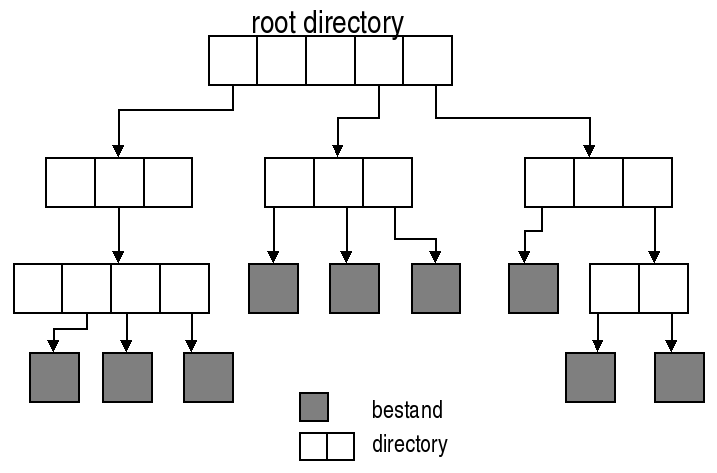
\includegraphics[width=75mm]{images/fig0401.png}
\end{center}
\caption{Boomstructuur}
\label{boomstructuur}
\end{figure}

\TODO{Figuur op slide 27 ch8.ppt van silberschatz toevoegen}

Om segmentatie effici\"ent te laten werken, is ondersteuning van de hardware
vereist. In het geval van de Intel x86-processor vertaalt zich dat naar de
volgende componenten:

\begin{itemize}
\item{Descriptor} Een descriptor is een gegevensstructuur die
een segment beschrijft. Het bevat onder andere het beginadres van het segment en
de lengte van het segment.
\item{Descriptorentabel} Er kunnen meerdere
programma's tegelijkertijd in het geheugen geladen zijn, en elk programma kan
meerdere segmenten hebben. Al de descriptoren die bij deze segmenten horen,
staan opgeslagen in de descriptorentabel. Deze tabel staat ergens in het
werkgeheugen opgeslagen en kan maximaal 8192 descriptoren bevatten.
\item{Segmentselector} Om een bepaalde descriptor uit de descriptorentabel aan
te duiden, kunnen we een getal gebruiken dat het volgnummer van de descriptor in
de tabel voorstelt. Dit getal noemen we een segmentselector.
\item{Segmentregister} De processor voorziet zes registers die tijdens de
uitvoering van een programma kunnen gebruikt worden om informatie over de
segmenten op te zoeken. Deze registers bevatten segmentselectors, waarmee de
processor dan naar de descriptorentabel kan gaan om de informatie van het
segment uit te lezen.
\end{itemize}

Wanneer een besturingssysteem een proces selecteert om uit te voeren, zullen de
segmentregisters ge\"initialiseerd worden met de correcte segmentselectors die
bij het programma horen. Bijvoorbeeld, in segmentregister \texttt{ds} komt de segmentselector
van de descriptor die het datasegment van de applicatie beschrijft.

Wanneer een applicatie een een instructie oproept die het geheugen aanspreekt, zal de instructie telkens de gewenste verplaatsing \'en het gewenste segment bevatten. Bijvoorbeeld, de instructie \texttt{mov al, [ds:1234]} haalt de byte op uit het geheugen die staat in het datasegment op verplaatsing 1234. Bij de uitvoering van deze instructie zal de processor een adresberekening doen. Eerst wordt door middel van de segmentselector in segmentregister \texttt{ds} de gevraagde descriptor opgehaald uit de descriptorentabel. De verplaatsing wordt vergeleken met de grootte van het segment; indien de gevraagde verplaatsing groter is zal de processor een fout genereren. Uiteindelijk zal bij de verplaatsing de basis opgeteld worden, om zo het fysieke adres te krijgen dat uit het werkgeheugen moet opgehaald worden.

\TODO{figuur i.v.m. adresberekening toevoegen}

Segmentatie heeft een aantal belangrijke voordelen. Zo kan een programma een groter stuk geheugen aanspreken dan dat de woordgrootte van de processor toelaat. Bijvoorbeeld, op een 16-bit processor bestaat een verplaatsing uit 16 bits. Dit wil zeggen dat de maximum grootte van een segment 2\textsuperscript{16} of 65536 bytes is. Wanneer er meer geheugen beschikbaar is, dan kan de applicatie gebruik maken van meerdere segmenten die elk een ander stuk fysisch geheugen beslaan.

De verschillende segmenten van een programma kunnen ook andere toegangsrechten krijgen. Zo kan het codesegment bijvoorbeeld allen-lezen gemaakt worden, en het datasegment niet-uitvoerbaar. Dit is van belang om er voor te zorgen dat bepaalde softwarefouten niet uitgebuit kunnen worden door een aanvaller.

Aangezien er enkel met verplaatsingen gewerkt wordt, is het programma verplaatsbaar in het geheugen. Elke keer dat het programma opgestart wordt, kan het ergens anders in het geheugen ingeladen worden. Ook kan hetzelfde programma meerdere keren in het geheugen staan. Deze eigenschap zorgt er voor dat het geheugenbeheer een stuk geavanceerder kan verlopen. Zo kan het besturingssysteem bij het inladen van het programma de meest-optimale plaats in het geheugen voor het programma zoeken. Wanneer een programma twee keer gestart wordt, kan het besturingssysteem er ook voor kiezen om bijvoorbeeld het codesegment te delen.

Het grootste nadeel van segmentatie heeft te maken met \emph{externe fragmentatie}. Net zoals bij het beheer van aaneengesloten bestanden, kunnen er bij segmentatie gaten vallen in het geheugen. Wanneer een klein segment verwijderd wordt, kan het stuk vrij geheugen te klein zijn om er een nieuw (groter) segment in te steken. Naarmate de tijd vordert, kan dit oplopen tot een aanzienlijk stuk van het geheugen dat niet meer gebruikt kan worden.

Een tweede nadeel is dat de segmenten van een programma altijd in hun geheel moeten worden ingeladen in het geheugen, ook al wordt er slechts een deel van het segment daadwerkelijk actief gebruikt.

\section{Paginatie}

Een manier om de twee nadelen van segmentatie op te lossen, is door te werken met \emph{pagina's} in plaats van segmenten. Een pagina is een stuk geheugen met een vaste grootte (bijv. 4KB). Een programma kan dan opgedeeld worden in meerdere pagina's. Het werkgeheugen wordt op een gelijkaardige manier opgedeeld in \emph{frames}; dit zijn blokken die dezelfde grootte hebben als een pagina. Wanneer een programma dan in het geheugen geladen wordt, moet het besturingssysteem de pagina's van het proces inladen in frames van het werkgeheugen die nog vrij zijn. De volgorde van de pagina's in een proces en de frames in het werkgeheugen staat volledig los van elkaar. Zo moeten opeenvolgende pagina's van een proces niet per se in opeenvolgende frames van het werkgeheugen gestoken worden.

\TODO{figuur?}

Deze manier van werken vermijdt externe fragmentatie omdat de frames die vrij komen steeds kunnen worden hergebruikt voor pagina's van nieuwe processen. Dit komt omdat de pagina's van alle processen steeds dezelfde grootte hebben. Omdat een proces opgedeeld moet worden in blokken, kan er zich echter wel \emph{interne fragmentatie} voordoen. Dit is het geheugen dat verloren gaat omdat een programma soms niet exact past in een bepaald aantal blokken. In dat geval zullen een aantal bytes van het laatste blok niet gebruikt worden. Gemiddeld gezien verliezen we een halve blok per programma aan deze interne fragmentatie. Programma's hoeven ook niet meer in hun geheel ingeladen te worden. Enkel de pagina's die nodig zijn moeten in het werkgeheugen te staan.

Wanneer een programma een adres gebruikt, wordt dat opgesplitst in twee delen: een \emph{paginanummer} en een \emph{offset}. Stel dat we werken met 32-bit adressen en pagina's van 4KB. Om elke byte van een 4KB-pagina te kunnen adresseren, zal de offset moeten bestaan uit 12 bits ($2^{12} = 4096$). De resterende 20 bits van het adres stellen dus het paginanummer voor, wat betekent dat er in ons voorbeeld maximaal $2^{20} = 1048576$ pagina's zijn. Aangezien deze adressen ge\"interpreteerd moeten worden en dus niet rechtstreeks overeenkomen met een adres in het werkgeheugen, noemen we ze \emph{virtuele adressen}.

Per proces maakt het besturingssysteem ook een \emph{paginatabel} (of \emph{page table}) aan. In deze tabel wordt de mapping tussen de pagina's van het proces en de frames van het werkgeheugen bijgehouden. Aangezien elk proces een andere paginatabel heeft, moet de CPU weten welke tabel hij wanneer moet gebruiken. De processor maakt hier een speciaal register voor beschikbaar, dat door het besturingssysteem beheerd wordt. Dit register wijst te allen tijde naar het adres van de actieve paginatabel. Wanneer het besturingssysteem een nieuw proces actief maakt, moet het dus de waarde in dit register aanpassen.

\TODO{Figuur 8.3 vanuit sliberschatz slide 16}

\subsection{Two-level page table}

Als we met hetzelfde voorbeeld van een computer met 32-bit adressen en 4KB pagina's verder gaan, dan kunnen we berekenen hoe groot een page table wordt. In een page table moet voor elk frame in het geheugen een \emph{page table entry} bijgehouden worden. Aangezien er $2^{20}$ frames zijn, moeten er dus evenveel entries beschikbaar zijn. Op de x86-processor is een page table entry 4 bytes groot, dus dan kunnen we berekenen dat een volledige page table 4MB groot is. Merk op dat elk proces een aparte page table heeft, en er dus voor elk proces 4MB geheugen gealloceerd moet worden, ook al gebruikt het proces slechts een klein stuk geheugen.

Om page tables effici\"enter in het geheugen op te slaan, kunnen we gebruik maken van een \emph{two-level page table}. Er wordt dan gebruik gemaakt van een hi\"erarchische structuur zoals beschreven in Figuur \TODO{ref figuur} waarbij een \emph{page directory} links bevat naar verschillende (kleinere) page tables. Niet elke link van de page directory moet in gebruik zijn; indien het programma weinig geheugen gebruikt, is \'e\'en link misschien al voldoende. Per proces is er slechts \'e\'en page directory. De processor weet waar die tabel in het geheugen staat, omdat het besturingssysteem het adres ervan in het speciale register \texttt{CR3} (van \emph{control register 3}) zet.

In dit geval wordt het 32-bit adres opgesplitst in 3 stukken: 12 bits voor de offset binnen de pagina, 10 bits die het paginanummer voorstellen en 10 bits die de index binnen de page directory voorstellen. Hieruit kunnen we afleiden dat in een page table en de page directory slechts $2^{10} = 1024$ entries kunnen.

\TODO{figuur van x86 page table}

Een programma dat heel veel geheugen gebruikt, zal elke entry in de page directory gebruiken. Er zullen dus 1024 page tables gebruikt worden die elk 4KB groot zijn (= 4 bytes * 1024 entries per page table). Wat het geheugengebruik betreft is in dit geval de grootte van de two-level page table vergelijkbaar met de grootte van het vorige systeem waar er slechts \'e\'en page table per proces was.

Het voordeel van de two-level page table is pas te zien wanneer de applicatie weinig geheugen gebruikt. In dit geval gebruikt de applicatie slechts \'e\'en kleine page table, wat neerkomt op een geheugengebruik van 8KB (= 4KB voor de page table en 4KB voor de page directory). Dat is aanzienlijk minder dan de 4MB die nodig zou zijn zonder een two-level page table.

\subsection{Multi-level page table}\label{multi-level-page-table}

Een two-level page table werkt goed voor een processor met een 32-bits geheugenruimte, maar het systeem schaalt niet zo goed naar 64 bits. Stel dat we een two-level page table willen toepassen op een 64-bit processor en dat we pagina's van 4KB gebruiken. Van de 64 bits in een adres, worden 12 bits gebruikt voor de offset binnen in een pagina. De resterende 52 bits kunnen dan opgesplitst worden voor de offset van de page directory en het paginanummer. Als we de bits evenredig zouden verdelen, da zouden we 26 bits voor de page directory kunnen gebruiken en 26 bits voor het paginanummer. Dit wil echter zeggen dat zowel de page directory als de page tables $2^{26} = 67108864$ entries moeten kunnen bevatten. Als we er van uit gaan dat de entries in de page directory en de page tables elk 8 bytes groot zijn, dan zouden we hier spreken over een minimaal geheugengebruik van 1GB per proces. Dat is natuurlijk niet realistisch.

De Intel x86-64 processor gebruikt dan ook geen two-level page table, maar een four-level page table\footnote{De Intel x86-processor ondersteunt ook three-level page tables, wat \emph{Physical Address Extension (PAE)} genoemd wordt.}. Figuur \TODO{figuur toevoegen} geeft een schematische voorstelling van deze structuur. Van het 64-bit adres worden 9 bits gebruikt als offset voor de \emph{page map level-4 table}. Deze tabel bevat wijzers naar \emph{page directory pointer tables}, die op hun beurt wijzers bevatten naar \emph{page directory tables}. Deze page directory tables verwijzen dan naar de page tables van het proces. Merk op dat van het 64-bit adres slechts 48 bits gebruikt worden. De overige 16 bits kunnen later gebruikt worden, wanneer een computer meer dan $2^{48} bytes = 256TB$ aan werkgeheugen heeft. Per proces is er slechts \'e\'en page map level 4 waarvan het adres in het speciale register \texttt{CR3} staat.

Een proces dat weinig geheugen gebruikt, heeft slechts \'e\'en page map level-4, page directory pointer, page directory en page table nodig. Elk van deze gegevensstructuren zijn 4KB, dus in totaal wordt er slechts 16KB geheugen gebruikt om te beschrijven welke frames het proces bezit.

\TODO{Figuur toevoegen van 4-level x64 page table}

Het converteren van een \emph{logisch adres} (d.i. een adres zoals een programma het gebruikt) naar een fysiek adres is zeker niet triviaal. Wanneer de processor voor de instructie \texttt{mov al, [ds:229504h]} het fysieke adres moet berekenen dat overeenkomt met het gevraagde logische adres 229504h, dan moet hij de volgende stappen ondernemen:

\begin{enumerate}
\item{\textbf{Offsets berekenen}} De bits van het hexadecimale adres worden opgesplitst in de verschillende offsets. Voor het adres 229504h geeft dit de volgende resultaten (in decimaal):
    \begin{enumerate}
    \item{Offset in pagina:}\label{PO} 1284
    \item{Page table index:}\label{PTE} 41
    \item{Page directory index:}\label{PDE} 1
    \item{Page directory pointer index:}\label{PDPE} 0
    \item{Page map level 4 index:}\label{PML4} 0
    \end{enumerate}
\item{\textbf{Page map entry zoeken}} De processor gebruikt het adres in register \texttt{CR3} om in het werkgeheugen de page map level 4-tabel te lokaliseren. In deze tabel gebruikt hij de index die hij in stap~\ref{PML4} berekend heeft om de jusite page map level 4 entry (PML4E) op te zoeken. In deze entry zit dan het adres van de page directory pointer tabel die gebruikt moet worden.
\item{\textbf{Page directory pointer entry zoeken}} In de page directory pointer-tabel wordt dan de entry gezocht die overeenkomt met de index die werd berekend in stap~\ref{PDPE}. Deze entry bevat dan het adres van de page directory die gebruikt moet worden.
\item{\textbf{Page directory entry zoeken}} In de page directory-tabel wordt de entry gezocht die overeenkomt met de index uit stap~\ref{PDE}. In deze entry vinden we het adres van de page table.
\item{\textbf{Page table entry zoeken}} In de page table zoeken we de entry die de informatie bevat over de pagina met het volgnummer uit stap~\ref{PTE}. Deze entry bevat dan het adres van het frame in het werkgeheugen waar de pagina zich bevindt.
\item{\textbf{De gevraagde byte ophalen}} Nu we weten waar de pagina zich in het geheugen bevindt, kunnen we hier de berekende offset (stap~\ref{PO}) bij optellen om uiteindelijk het adres te krijgen van de gevraagde byte.
\end{enumerate}

De bovenstaande berekening moet gebeuren voor \'elke instructie die een adres gebruikt. Het spreekt voor zich dat deze berekening z\'e\'er snel moet uitgevoerd kunnen worden. Alhoewel de page map, page directory pointer, page directory en page table allen in het (trage) werkgeheugen staan, is dit gelukkig geen groot probleem: omdat ze zo vaak opgevraagd worden blijven ze in de processor cache staan. Hierdoor kunnen de tabellen zeer snel uitgelezen worden. Om het een en ander nog te versnellen, voorziet de processor typisch ook een \emph{translation lookaside buffer (TLB)}. Deze component werkt op een gelijkaardige manier als de cache, maar dient expliciet om de resultaten die berekend werden a.d.h.v. de bovenstaande stappen op te slagen voor later hergebruik.

\section{Segmentatie \'en paginatie}

Paginatie laat complexere geheugenbeheerscenario's toe, dus je zou kunnen zeggen dat paginatie beter is dan segmentatie. Uit compatibiliteitsoverwegingen wordt op de Intel x86-architectuur echter zowel segmentatie als paginatie ondersteund\footnote{De Intel x86-64 architectuur die momenteel de standaard is voor desktops en laptops ondersteunt g\'e\'en segmentatie meer, maar enkel paginatie (zoals beschreven in sectie~\ref{multi-level-page-table}).}. Schema~\TODO{figuur} illustreert hoe dit werkt.

\TODO{figuur 3-1 van intel developer manual (toledo)}

Stel dat het actieve programma de instructie \texttt{mov al, [ds:0982CA0Fh]} wil uitvoeren en dat het datasegment (= segment \texttt{ds}) begint op adres 10000000h). Uit figuur~\TODO{ref fig} kunnen we afleiden dat de processor voor de adresberekening de volgende stappen moet volgen:

\begin{enumerate}
\item{\textbf{Descriptor ophalen}} De instructie specifieert dat segment \texttt{ds} gebruikt wordt. De segmentselector wordt uit segmentregister \texttt{ds} gehaald en de overeenkomstige descriptor wordt opgezocht in de globale descriptorentabel. Deze descriptor bevat het basisadres van het segment (10000000h).
\item{\textbf{Logisch adres berekenen}} Het logische adres wordt berekend door bij het basisadres van het segment de verplaatsing (die in de instructie staat) op te tellen. Het resultaat is het logische adres 1982CA0Fh
\item{\textbf{Offsets berekenen}} De bits van het logische adres worden opgesplitst in de verschillende offsets. Voor het adres 1982CA0Fh geeft dit de volgende resultaten (in decimaal):
    \begin{enumerate}
    \item{Offset in pagina:}\label{PO86} 2575
    \item{Page table index:}\label{PTE86} 44
    \item{Page directory index:}\label{PDE86} 102
    \end{enumerate}
\item{\textbf{Page directory entry zoeken}} In de page directory-tabel wordt de entry gezocht die overeenkomt met de index uit stap~\ref{PDE86}. In deze entry vinden we het adres van de page table.
\item{\textbf{Page table entry zoeken}} In de page table zoeken we de entry die de informatie bevat over de pagina met het volgnummer uit stap~\ref{PTE86}. Deze entry bevat dan het adres van het frame in het werkgeheugen waar de pagina zich bevindt.
\item{\textbf{De gevraagde byte ophalen}} Nu we weten waar de pagina zich in het geheugen bevindt, kunnen we hier de berekende offset (stap~\ref{PO86}) bij optellen om uiteindelijk het adres te krijgen van de gevraagde byte.
\end{enumerate}

\section{Virtueel geheugen}

De technieken die in de vorige secties beschreven werden, kunnen gebruikt worden om aan complex geheugenbeheer te doen. Zo kunnen besturingssystemen bijvoorbeeld het concept van \emph{virtueel geheugen} (of \emph{virtual memory}) aanbieden. Hierbij zorgt het besturingssysteem dat het voor elke applicatie \emph{lijkt} alsof ze de hele geheugenruimte ter beschikking hebben. Zo wordt bijvoorbeeld de code van elk proces op de lage adressen geplaatst en de stapel op de hoge adressen. Achter de schermen zorgt het besturingssysteem er d.m.v. paginatie voor dat al deze \emph{virtuele adressen} gemapped worden op andere fysieke adressen, maar vanuit het standpunt van de applicatie ziet zijn geheugenruimte er steeds hetzelfde uit.

Het concept van virtueel geheugen kan ge\"implementeerd worden met behulp van paging \emph{of} segmentatie. In de rest van deze tekst gaan we er van uit dat paging gebruikt wordt, aangezien dit het meest gebruikt wordt in de praktijk en ook geavanceerdere scenario's toelaat.

\subsection{Demand Paging}

In Hoofdstuk~\ref{procesbeheer} werd gezegd dat elk programma dat uitgevoerd wordt in het geheugen moet staan. Het is natuurlijk waar dat een processor enkel instructies kan uitvoeren die in het geheugen staan, maar in de praktijk is het zelden het geval dat elke instructie van een applicatie effectief uitgevoerd wordt (en dus in het geheugen moet staan). Vaak zit er in een programma ook heel wat code voor functionaliteit die amper gebruikt wordt. We kunnen het inladen van het programma dus versnellen door enkel de code in het geheugen te laden die daadwerkelijk gebruikt wordt.

Een techniek die hiervoor gebruikt kan worden is \emph{demand paging}. Een programma wordt in pagina's verdeeld, en enkel de pagina's waar vraag achter is worden in het geheugen geladen. Zo worden enkel pagina's in het geheugen geladen die gebruikt worden; niet-gebruikte pagina's zullen nooit ingeladen worden. Dit heeft een positieve impact op het aantal I/O-operaties dat het besturingssysteem moet doen om het programma in te laden waardoor er minder geheugen nodig is en de computer sneller reageert.

Demand paging vereist wel een aantal hardware-aanpassingen om alles effici\"ent te laten verlopen. De page table entries moeten aangepast worden zodat ze een bit bevatten die aangeeft of de pagina in het geheugen geladen is of niet. Indien dit wel het geval is, dan kan de processor uit de page table entry het adres van het frame ophalen waar de pagina staat. Als de pagina echter niet ingeladen is, dan zal de processor een zogenaamde \emph{page fault} genereren. Dit is een interne interrupt die door het besturingssysteem zal opgevangen worden. Het actieve programma dat de niet-ingeladen pagina opvroeg wordt onderbroken, de interrupt handler laadt de gevraagde pagina in het geheugen, en het programma wordt hervat.

\TODO{misschien slide 15 van chapter 9 silberschatz toevoegen}

\subsection{Swapping}

Zolang er frames in het geheugen vrij zijn, kunnen er nieuwe pagina's ingeladen worden door het demand paging-systeem. Er rijst dan echter de vraag wat er gebeurt indien er zich een page fault voordoet, en het geheugen helemaal vol zit. Het besturingssysteem zal dan niet zomaar een nieuwe pagina kunnen inladen. Omwille van de flexibiliteit van paging hoeft dit echter geen probleem te zijn: het besturingssysteem kan simpelweg een ingeladen pagina (eventueel van een ander proces) uit het geheugen verwijderen, waardoor er plaats vrijkomt. Deze techniek noemt men \emph{swapping}.

De verwijderde pagina mag natuurlijk niet zomaar weggegooid worden. Het programma waartoe de pagina hoort kan ze mogelijk later nog nodig hebben. Daarom worden de verwijderde pagina's opgeslagen op een speciale plaats op de harde schijf: de \emph{swap file} (of soms een \emph{swap partitie}). Toegang tot de swap file is natuurlijk veel trager dan het werkgeheugen, dus het besturingssysteem zal proberen om zo weinig mogelijk te swappen.

De manier waarop het besturingssysteem kiest welke pagina verwijderd moet worden, is belangrijk. Zo mag de pagina best niet in de nabije toekomst terug gebruikt worden. Het besturingssysteem kan die natuurlijk nooit met zekerheid weten, maar kan wel gokken hoe `populair' een pagina is. Een pagina van een hoge-prioriteitsproces is bijvoorbeeld al een minder goede kandidaat om uit te swappen dan een pagina van een lage-prioriteitsproces.

Swapping laat toe om meer geheugen te gebruiken dan dat er fysisch in de computer zit. Indien de computer 2GB werkgeheugen heeft en een swap file van 1GB, dan kan het besturingssysteem voor 3GB aan data in het geheugen steken. Op eender welk moment zal er natuurlijk maximaal 2GB echt in het werkgeheugen aanwezig zijn; de rest zit dan in de swap file.

\subsection{Sharing}

Een interessante manier om geheugen uit te sparen is door pagina's tussen processen te delen. Van een programma dat twee keer opgestart wordt, moet er slechts \'e\'en keer het codesegment in het geheugen geplaatst worden. Verschillende programma's gebruiken vaak ook dezelfde bibliotheken die kunnen gedeeld worden.

Conceptueel is het delen van pagina's eenvoudig: het besturingssysteem moet in de verschillende page tables van de processen gewoon hetzelfde frame mappen. Beide processen kunnen dan aan de data van dat frame aan. Deze techniek kan perfect gebruikt worden voor effici\"ente inter-proces communicatie. Het ene proces kan bijvoorbeeld data schrijven naar dat frame, wat het andere proces dan kan uitlezen.

Deze eenvoudige manier van delen is echter minder geschikt voor het delen van code. Het is natuurlijk niet wenselijk dat kwaadaardige software de pagina van een gedeelde bibliotheek kan aanpassen die ook door andere programma's gebruikt wordt. Een aanvaller zou zo een bepaalde functie in een bibliotheek kunnen aanpassen om zo de controle van andere programma's over te nemen. Om dit probleem op te lossen, heeft elke pagina \emph{toegangsrechten}. Hiermee kan het besturingssysteem pagina's als \emph{alleen-lezen} (\emph{read only}) markeren, of \emph{niet-uitvoerbaar} (\emph{no-execute}). Pagina's van gedeelde bibliotheken zijn alleen-lezen, waardoor iedereen ze kan lezen en uitvoeren, maar niet aanpassen. Pagina's van de stapel, bijvoorbeeld, zijn meestal niet-uitvoerbaar; de stapel bevat dan ook geen programmacode.

De meeste besturingssystemen reserveren ook een stuk van de virtuele geheugenruimte om pagina's te mappen die de code van de systeemroutines bevatten. Elk proces moet (dezelfde) systeemroutines kunnen oproepen, dus is het logisch dat de code van deze routines gedeeld wordt.

\subsection{Thrasing}

Wanneer van een proces veel pagina's niet in het werkgeheugen geladen zijn, zal het proces vaak onderbroken moeten worden om te swappen. Wanneer het werkgeheugen echter klein is, kan het voorvallen dat de pagina's die uitgeswapt worden snel terug gebruikt worden. In dit geval gaat er veel tijd verloren aan het in- en uitswappen van pagina's. De processor wordt hierdoor te weinig gebruikt (omdat alle processen aan het wachten zijn op pagina's). Wanneer een proces veel tijd verliest aan het in- en uitladen van pagina's, zegt men dat het aan het \emph{trashen} is. Meestal is dit ook niet gelimiteerd tot \'e\'en proces, maar wordt het ganse systeem be\"invloed. Een effectieve manier om thrashing op te lossen wanneer het zich voordoet, is door programma's af te sluiten en zo geheugen vrij te maken.






